% !TEX root = ../../numb3rs.tex
\newpage
\subsection{111: Sacrifice\label{111}}

In this episode the data from a murdered researcher's computer is recovered after being ``wiped''. After a review of the basics of magnetism and binary encoding, we will explore how the two are combined to store data on hard disk drives and how this data might be recovered after being overwritten with other data. \\

%%%%%%%%%%
\temph{Magnetism}
%%%%%%%%%%

	\begin{figure}[H]
	   \centering
	   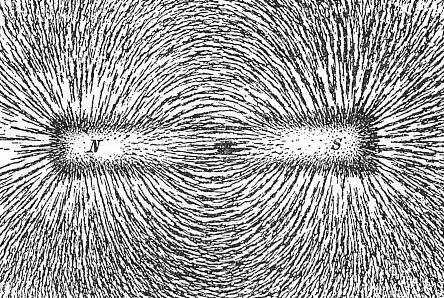
\includegraphics[width=0.5\textwidth]{season1/111/images/magnet.png} 
	\end{figure}

You have probably played with bar magnets, like the one on the right, before, discovering that they have two distinct poles and that like poles of two bar magnets repel while opposite attract. What you might have not realized is that magnetism originates at the subatomic level. Electrons (and other subatomic particles) have an intrinsic property misleadingly called spin; it does not refer to the particles actually spinning in the everyday sense of the word--it's more accurate to think of spin as a property of a particle akin to mass or charge. Nevertheless, as spinning a larger charged object creates a magnetic dipole (i.e. makes the spinning object produce a magnetic field), so does the spin of an electron make it behave like a tiny bar magnet. Additionally, when the electron also orbits an atom, this gives it another distinct magnetic dipole created by this orbiting, usually called the orbital dipole moment. The magnitude and axis of both of these magnetic moments can be expressed as \bref{vectors}{https://en.wikipedia.org/wiki/Coordinate_vector}; adding those up we get the total magnetic dipole contributed by one electron. If we sum up these dipoles for each electron in each atom of a small object, and they do not cancel each other out, then that object, like the bar magnet above, produces a magnetic field and is known as a magnet. \\

\fbox{\begin{minipage}{43em}
\begin{center} \large \dotuline{Activity 1}  \\ \end{center}
\begin{enumerate}[1.]
\item Use wikipedia or other internet resources to find out about the differences between diamagnetic, paramagnetic, and ferromagnetic elements.
\item What would happen if you take a bar magnet and break it in half near the midway point dividing the north and south poles? Can you use what you've read about ferromagnetism and the discussion above to explain why this happens?
\end{enumerate}
\end{minipage}} \vspace{0.2cm}

In addition to electrons producing magnetic fields by their spin and orbit around an atomic nucleus, moving electrons also create a magnetic field ``around'' the direction of motion, a phenomenon called electromagnetic induction. For instance, if a current flows through a straight wire, as on the right, a magnetic field is induced according to the \bref{right hand rule}{https://en.wikipedia.org/wiki/Right-hand_rule}. Such a magnetic field can be used to realign the polarity of ferromagnetic materials, allowing the possibility of storing information in magnetic alignment, which is the basis of digital storage media like hard drives and floppy disks. \\

	\begin{figure}[H]
	   \centering
	   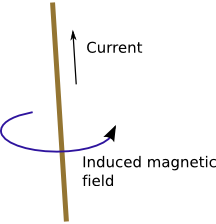
\includegraphics[width=0.3\textwidth]{season1/111/images/111(1).png} 
	\end{figure}

%%%%%%%%%%
\temph{Binary Encoding}
%%%%%%%%%%

Throughout history humans used symbols, whether pictures, pictograms, or alphabets, to communicate, replicate, and store information. What differentiates older ways of storing information in books or manuscripts from what happens when you select ``Save'' in your word processor is the form of the encoding. By encoding I mean the representation of information in a way different from its original form. These sentences, for instance, encode information that originally exists as ideas in my mind. Encryption is another example of encoding, as is compression. \\

\fbox{\begin{minipage}{43em}
\begin{center} \large \dotuline{Activity 2}  \\ \end{center}
\begin{enumerate}[1.]
\item Julius Caesar used a simple shift encoding to communicate with his generals. In this encoding a letter of the Roman alphabet was replaced by one appearing n after it, for some positive integer n, wrapping at the end of the alphabet to the beginning. Although Caesar originally used $n=3$, the most famous version of this scheme is rot13, in which $n=13$, so that A becomes N, B becomes O, etc. The next part of this activity is encoded in rot13. Decode and do it.
\item N fgnaqneq jnl gb rapbqr gur Ratyvfu nycunorg hfrq ol pbzchgref vf NFPVV, Nzrevpna Fgnaqneq Pbqr sbe Vasbezngvba Vagrepunatr. Vg rapbqrf rnpu yrggre nf n guerr-qvtvg ahzore. Ybbx hc na NFPVV gnoyr bayvar, naq qrpbqr gur jbeq va cneg 3 bs guvf npgvivgl.
\item 067 111 110 103 114 097 116 117 108 097 116 105 111 110 115 !
\end{enumerate}
\end{minipage}} \vspace{0.2cm}

Once we've encoded our alphabet as ASCII numbers, the next step is to encode these numbers using a series of blocks each with only two states, on or off, as in case of a ferromagnetic material which can be aligned along only one axis, with the north pole pointing either up or down. This is accomplished by converting ASCII codes into binary. \\

Note that $2008=8\cdot 10^0+0\cdot 10^1+0\cdot 10^2+2\cdot 10^3$. By writing ``2008'' in everyday use we mean for the digits to simply enumerate how many 1s, 10s, 100s, and 1000s are in the number. But if we look at it this way, a natural question arises: why use the powers of 10, instead of say, powers of 3 or 7? Indeed, there's absolutely no objective reason to chose 10--resulting in what's called the decimal or base 10 numerical system--over other possible bases. The Sumerians, for example, used base 60, hence the 60 seconds per minute, 60 minutes per hour. The following activity should give you a feel for how different bases work and how to convert from one to another.

\fbox{\begin{minipage}{43em}
\begin{center} \large \dotuline{Activity 3}  \\ \end{center}
Let $m_n$ denote the number $m$ in base $n$. For instance, $5_{10}=101_2=1\cdot 2^0+0\cdot 2^1+1\cdot 2^2$.
\begin{enumerate}[1.]
\item Here's an algorithm for converting from base 10 to base 4: take your number, say $103_{10}$, divide by 4, recording and discarding the remainder, in this case 3 ($103=4\cdot 25+3$). Divide the result by 4 again, recording and discarding remainder, rinse and repeat until you get 0. ($25=4\cdot 6+1$, $6=4\cdot 1+2$, $1=4\cdot 0+1$). Concatenate the remainders in reverse order to get the number base 4, $1213_4=103_{10}$. Why does this algorithm work?
\item Design an algorithm to convert from base 4 to base 16.
\end{enumerate}
\end{minipage}} \vspace{0.2cm}

\fbox{\begin{minipage}{43em}
\begin{center} \large \dotuline{Activity 4}  \\ \end{center}
Besides binary (base 2), another common base used by computer scientists and programmers is hexadecimal, or base 16. Why do you think this is? (Hint: see part 2 of the previous activity).
\end{minipage}} \vspace{0.2cm}

%%%%%%%%%%
\temph{Hard Drives and Data Recovery}
%%%%%%%%%%

Your computer \bref{hard drive}{https://en.wikipedia.org/wiki/Hard_disk_drive} consists of layered, circular platters of ferromagnetic material that quickly spin while read/write heads hover above. Those read/write heads are able to read and change the magnetic polarity of tiny areas on a platter's surface. The more such areas are squeezed onto the platters, the larger the storage capacity of the hard drive. The reading and writing operations are accomplished using the principle of electromagnetic induction discussed previously: a current passing through the tip of the head is used to change the polarity of the area below, and the reverse effect--the appearance of a current in response to a changing magnetic field--is used to measure the existing magnetic alignment. \\

Normally, when you delete something in Windows or on a Mac (and in most modern Linux systems), the files are not deleted but their records are moved from the folder they originally resided into a designated ``Trash/Recycle Bin'' area. During this operation the actual data on the disk is left untouched, and the files are easily recoverable from trash. If you empty the trash bin, the records of the files get destroyed: the filesystem designates the physical space in which the file resides as empty. However, the actual file, the bits encoded in the magnetic alignment, do not get realigned in any way. Thus the information is actually kept completely intact until it is overwritten, there's just no way to readily access or restore it. However, restoring such non-overwritten files is not particularly difficult; there exist both commercial and free software tools to do exactly that. Things get much more interesting, and contentious, when it comes to restoring information that has been overwritten one or more times. \\

The most important paper on this subject is Peter Gutmann's \bref{Secure Deletion of Data from Magnetic and Solid-State Memory}{https://www.cs.auckland.ac.nz/~pgut001/pubs/secure_del.html}. It describes the following method of recovering overwritten data. Suppose we zoom onto a hard drive's surface and discover that the initial alignment within each area are as illustrated below. \\

	\begin{figure}[H]
	   \centering
	   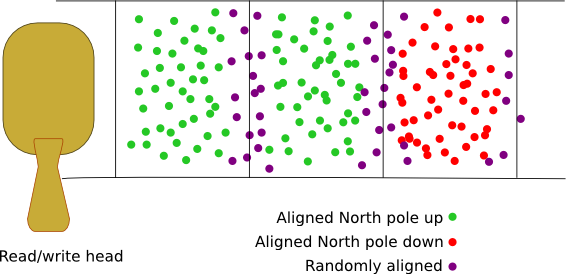
\includegraphics[width=0.5\textwidth]{season1/111/images/111(3).png} 
	\end{figure}

Suppose we now overwrite the middle area: change the alignment to point down. \\

	\begin{figure}[H]
	   \centering
	   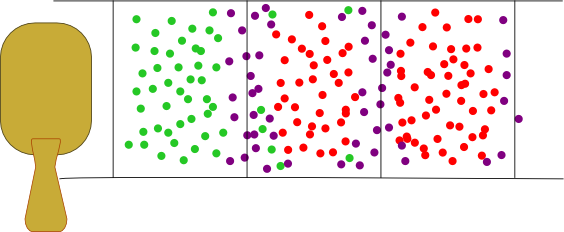
\includegraphics[width=0.5\textwidth]{season1/111/images/111(4).png} 
	\end{figure}

Due to microscopic imperfections in the read/write head and tiny imprecisions in its movements, there will be a small band of the previous up aligned particles left, separated from the new down aligned particles by a thin buffer band of randomly aligned particles. Overwriting the same area again will create additional microscopic bands of molecules aligned according to the previous magnetic alignment. These bands will trace out the history of previous magnetic alignment of this area of the hard disk, and when examined with a powerful \bref{electron microscope}{https://en.wikipedia.org/wiki/Electron_microscope} can be read. Naturally, the more times an area is overwritten, the ``fainter'' the outer bands become and the harder it becomes to reconstruct long erased alignments. \\

This is the theory presented in the paper above, much of which has been confirmed. However, the most important and contentious claim made in the paper, that all this can be done quickly and efficiently enough to actually recover any nontrivial amount of overwritten data, and that such techniques are being used by intelligence agencies, remains unproven. Nonetheless, many software packages have been written which wipe files by overwriting the areas in which they are located repeatedly, thus making it virtually impossible to detect the original alignment. \\

